% vim: ts=4 sts=4 sw=4 et tw=80
\chapter{效率推进器}
\label{chap:production_boosters}

\marginpar{73}
在这一章我们将会看到, 即使是一些小小的改动, 也可以极大地促进 Vim 的工作效率.
有些技巧是由 Vim 的特性提供的, 另外一些则需要用户自已编写一些脚本.

无论你把 Vim 当成一个修改配置文件的小工具, 还是把它用作某个大型开发项目的主要
编辑器, 你都可以发现本章介绍的方法可以极大地促进 Vim 的使用效率.

这一章讨论的主题包括:
\begin{itemize}
    \item 使用模版文件的模版
    \item 使用缩写的模版
    \item 使用已知单词与 tag list 的自动补全
    \item 使用 omnicompletion 的自动补全
    \item 宏与宏录制
    \item 使用会话
    \item 使用会话的项目管理
    \item 寄存器与撤消分支
    \item 折叠
    \item 使用 \texttt{vimdiff} 分析差异
    \item 使用 \texttt{netrw} 来随时随地地打开文件
\end{itemize}

阅读完这一章之后, 用户使用 Vim 的工作效率应该可以提高好几个百分点.
\marginpar{74}

\section{使用模版}
\label{sec:using_templates}

无论编辑的是哪一种类型的文件, 当打开一个新文件时, 总有一些基础性的工作需要完成.
手动完成这些基础工作是一件非常乏味的事件, 更讨厌的是每次打开一个新文件时, 都
要重新再做一遍. 所以说干嘛要花这么多的时间, 来做一件使用模版就可以完成的事情?

在接下来的两节, 我们将会看到一些不同类型的模版. 其中一些模版特定于文件类型, 另
外一些则会使用用户的输入来触发小内容模版 (比如, 程序员经常用到的代码片断).

\subsection{使用模版文件}
\label{subsec:using_template_files}

每次打开一个新文件时, 用户做的第一件事经常是输入某些头部信息, 当然, 所要输入的
信息取决于文件的类型. 比较常见的例子包括:
\begin{itemize}
    \item 在新的 HTML 文件中添加基本结构 (\texttt{<html>}, \texttt{<head>},
        \texttt{<body>}).
    \item 在所有的 C 文件添加头部信息, 在文件 \texttt{main.c} 中添加
        \texttt{main()} 函数.
    \item 在 Java 文件中添加主类.
\end{itemize}
除了这些, 你应该还能想到其他一些例子.

那么, 我们怎么才能创建一个模版文件? 不妨让我们用 HTML 文件作为例子来进行讲解.
这种文件的结构是静态的, 因此非常适合用模版来处理. HTML 模版的内容是:
\begin{vimcode}
<html>
    <head>
        <title></title>
            <meta name="generator" content="Vim" />
            <meta name="author" content="Kim Schulz" />
    </head>
    <body>
        <p>Content goes here...</p>
    </body>
</html>
\end{vimcode}
我们在 \texttt{VIMHOME} 目录下创建一个新目录 \texttt{templates/}, 并把上面的
模版文件保存到这个目录中, 假设我们把模版文件命令为 \texttt{html.tpl}.
\marginpar{75}
现在, 第一个模版已经准备就绪, 不过, 当我们创建一个新的 HTML 文件时, 需要加载
模版文件, 为了完成加载, 把下面这行命令添加到 \texttt{vimrc} 中:
\begin{vimcode}
:autocmd BufNewFile *.html 0r $VIMHOME/templates/html.tpl
\end{vimcode}
这个命令可以确保当我们新建一个 \texttt{*.html} 文件时, 模版文件的内容会自动加
载到新文件中. 于是, 当我们开始编辑新文件前, 文件中就已经包含了模版的内容.

本来这样做没什么问题, 但是当添加的模版文件越来越多时, 我们可能会越来越讨厌每
次都要往 \texttt{vimrc} 中添加一行加载命令. 所以, 让我们把加载模版的命令写得
更灵活一点:
\begin{vimcode}
:autocmd BufNewFile * silent! 0r $VIMHOME/templates/%:e.tpl
\end{vimcode}
命令的功能是: 无论何时打开一个新文件, Vim 就在模版目录中搜索以文件扩展名命名
的模版. 比如, 创建一个 \texttt{index.html} 文件时, Vim 就在
\texttt{\$VIMHOME/templates/} 中搜索名为 \texttt{html.tpl} 的模版文件.

如果没有找到指定的模版, Vim 就创建一个空文件.

让我们把模版写得更完善一点: 添加对占位符 (占位符指的是你将要添加文本的地方) 的
支持. 一个占位符看起来可以非常得与众不同, 这取决于你, 笔者通常把它们显示成类似
于 \texttt{<+KERWORD+>} 的形式. 如果我们在前面的 HTML 模版中添加上占位符,
模版的内容就变成了:
\begin{vimcode}
<html>
    <head>
        <title><+TITLE+></title>
            <meta name="generator" content="<+GENERATOR+>" />
            <meta name="author" content="<+AUTHOR+>" />
    </head>
    <body>
        <p><+CONTENT+></p>
    </body>
</html>
\end{vimcode}

现在, 我们已经准备好了占位符, 接下来的工作就是在占位符之间跳转. 为了让跳转更加
方便, 我们把跳转命令添加到 \texttt{vimrc} 中. 我们想要把组合键 \key{Ctrl+j}
映射到跳转命令, 因为这样做的话便于在插入模式下使用, 组合键中 \texttt{j} (意
指 jump) 也更容易记忆. 映射组合键的命令是:
\begin{vimcode}
nnoremap <c-j> /<+.\{-1,}+><cr>c/+>/e<cr>
inoremap <c-j> <ESC>/<+.\{-1,}+><cr>c/+>/e<cr>
\end{vimcode}
\marginpar{76}
现在, 只需要按下组合键 \key{Ctrl+j}, 你就可以方便地跳转到文件中的下一个占位符,
输入文本, 然后再跳转到下一个占位符.

通过在占位符中添加关键字, 就可以提醒用户应该在占位符中输入什么样的内容.

\begin{warning}
可以通过命令 \texttt{match} 高亮显示占位符, 具体的设置命令是:
\verb'match Todo /<+.\++>/', 把这行命令添加到 \texttt{vimrc} 中 (可以把命令中的
\texttt{Todo} 替换成任意一种你喜欢的色彩组.
\end{warning}

\subsection{把缩写作为模版}
\label{subsec:abbreviations_as_templates}

在前面的小节里, 我们学习了如何为不同类型的文件制作模版. 那么, 现在就来介绍一下
如何为文件的内容制作模版.

在第 \ref{chap:personalizing_vim} 章, 我们简单地介绍了如何通过缩写来减少击键的
次数, 现在我们就把缩写应用到模版中. 回忆一下下面这个命令的作用:
\begin{vimcode}
:iabbrev match replace-string
\end{vimcode}
我们只想让上面的命令工作在插入模式, 这是因为模式模版本来就应该工作在插入模式下.
对于 C 文件来说, 一个常见的例子是:
\begin{vimcode}
:iabbrev <buffer> for( for (x=0;x<var;x++){<cr><cr>}
\end{vimcode}
无论我们在什么时候输入文本 \texttt{for(}, Vim 都会自动插入一段 \texttt{for} 循
环. \texttt{(} 可以防止手工输入的 \texttt{for} 循环被自动转换. 插入的内容看起
来就像:
\begin{vimcode}
for (x=0;x<var;x++){

}
\end{vimcode}

\begin{warning}
    缩写词左边的 \texttt{<buffer>} 把命令的作用范围限制在当前缓冲区内.
\end{warning}

正如你所看到的那样, 生成的代码模版是静态的. 为了让模版更灵活一点, 把前面一节介
绍的占位符应用进来.
\marginpar{77}
在这种情景下使用的占位符更像是一个跳转点, 因此我们把它们简化成 \texttt{<+++>}.
除此之外, 在插入模式模版之后, 我们需要在光标的下一个位置上放置一个占位符, 对于
前面的例子来说, 光标的下一个位置应该是左括号的右边.

为了实现这个目标, 我们引入 \texttt{!cursor!} 占位符, 命令的内容是:
\begin{vimcode}
iabbrev for( for(!cursor!;<+++>;<+++>){<cr><+++><cr>}<Esc>
    :call search('!cursor!','b')<cr>cf!:
\end{vimcode}
(上面的命令都在同一行上)

现在, 无论何时输入 \texttt{for(}, Vim 都会自动插入一段 \texttt{for} 循环, 然后 
把光标移动到占位符 \texttt{!cursor!} (当光标移过来时, 占位符上原来的内容会自动
被移除). 接下来, 你就可以方便地填写 \texttt{for} 循环的参数, 并用 \key{Ctrl+j}
跳转到下一个参数的位置.

也许你已经知道, 许多编程语言都有相同的主要结构 (比如 \texttt{for} 循环), 但是 
它们之间的差异导致了无法使用同一个模式模版. 让我们回过头来看一下手上已有的东西,
看看是否可以让它们识别文件类型.

在前面的一节里, 我们介绍了如何根据文件的扩展名来加载相应的模版文件, 具体的命令
是:
\begin{vimcode}
:autocmd BufNewFile * silent! 0r $VIMHOME/templates/%:e.tpl
\end{vimcode}
让我们对这个命令进行修改, 使得 Vim 可以根据文件的类型, 为我们的模式模版自动加
载适当的缩写.

为了能让命令更聪明一点, 我们把命令的功能用函数来实现. 函数的代码是:
\begin{vimcode}
function! LoadTemplate(extension)
    silent! :execute '0r $VIMHOME/templates/'. a:extension. '.tpl'
    silent! execute 'source $VIMHOME/templates/'.a:extension.'.patterns.tpl'
endfunction
\end{vimcode}
为了调用函数, 我们把 \texttt{autocmd} 修改成:
\begin{vimcode}
:autocmd BufNewFile * silent! call LoadTemplate('%:e')
\end{vimcode}
函数 \texttt{LoadTemplate} 在 \texttt{\$VIMHOME} 的 \texttt{templates} 子目录
下搜索两个文件: \texttt{EXTENSION.tpl} 与 \texttt{EXTENSION.patterns.tpl}.
其中 \texttt{EXTENSION} 表示当前打开着的文件的扩展名.
\marginpar{78}
第 1 个文件包含了特定文件类型的模版, 而第 2 个文件则包含了特定文件类型的缩写
命令. 如果没有找到对应的文件, 那么命令 \texttt{silent!} 就会抑制错误信息的输
出, 什么也不会显示出来.

现在, 模版文件中该包含什么样的内容完全由用户来决定.

\begin{warning}
    已经有人为 Vim 编写了大量的模版系统脚本, 其中大部分都是以本章介绍的概念为基础,
    但是增加了许多额外的功能. 除了这里介绍的之外, 如何用户还想要更多的模版选项,
    笔者推荐你看一下由 Gergely Kontra 编写的 mu-template, 可以到下面这
    个网址下载: \url{http://www.vim.org/scripts/script.php?script_id=222}.
\end{warning}

\subsection{snipMate 脚本}
\label{subsec:snippets_with_the_snipmate_script}

虽然已经有大量的模版系统脚本可供使用, 而且它们中的大部分都是以本章介绍的概念
为基础, 但是有时候对于特定的文件格式, Vim 还是没有提供足够的支持. 对于这些情况,
用户可以使用 snippet 脚本. Snippet 和用在模版中的缩写有点类似, 但是要更高级一
点.

如果你想在 Vim 中使用 snippet, 笔者推荐你看一下 snipMate 脚本, 下载地址是
\url{http://www.vim.org/scripts/script.php?script_id=2540}.

snipMate 可以让用户在不需要了解 Vim 脚本的前提下, 为自己的文件格式定义高级的
snippet.

假设用户想为 \texttt{for} 循环创建一个 snippet (在前面的一节里我们用的是 
\texttt{iabbrev}),  那就这样做:
\begin{vimcode}
snippet for
    for (${1:i} = 0; $1 < ${2:count}; $1${3:++}) {
        ${4:/* code */}
    }
\end{vimcode}
把上面这段文本写到一个文件中, 再把这个文件放到 \texttt{\$VIMHOME/snippets} 目
录下, 把文件命名为 \texttt{FILETYPE.snippet} (\texttt{FILETYPE} 表示文件类型,
比如 C 代码就是 \texttt{c}, PHP 代码就是 \texttt{php}).
\marginpar{79}
脚本的第一行表示开始一个新的 snippet, 当输入 \texttt{for} 并且后面再紧跟着一个
\key{Tab} 键时, 执行 snippet 脚本.

再接下来的一行是最神奇的, 脚本实际生成的代码看起来就像:
% FIXME
\begin{vimcode}
    for (i = 0; I < count; i++) {
        /* code */
    }
\end{vimcode}

snippet 被插入之后, 它把光标放在了第 1 个 \texttt{i} 的位置, 并切换到插入
模式, 因此你可以轻易地把 \texttt{i} 换成另一个变量. 现在, 最神奇的事情发生了,
% FIXME
当你把第 1 个 \texttt{i} 换掉之后, 第 2 个 \texttt{i} (后面带有 \texttt{++}
的那个) 也会被自动更新成新变量. 修改了 \texttt{i} 之后 (如果需要的话), 按下
\key{Tab} 键, 光标就会跳转到 \texttt{count}, 并再次切换到插入模式. 现在你可以
以同样的步骤来修改 \texttt{count} 并按下 \key{Tab} 键, 之后, 光标跳转到
\texttt{++}, 再按下 \key{Tab} 跳到 \texttt{/* code */}, 你可以在这里写下其他代
码.

在 snippet 的不同变量之间跳转, 简直不能再简单了.

snipMate 系统通过查找由 \texttt{\$\{NUMBER:INITIAL\_VALUE\}} 创建的特殊标记来进行
工作. 标记中的 \texttt{NUMBER} 指出了当你按下 \key{Tab} 时, 将要跳转到的序列.
如果 \texttt{NUMBER} 是 1, 那么光标会首先处在这个位置上, 如果 \texttt{NUMBER} 
是 3, 那么它就是按下两次 \key{Tab} 后光标所在的位置, 以此类推.
\texttt{INITIAL\_VALUE} 是在你修改 snippet 之前, 首先插入到 snippet 中的文本.
比如 \texttt{\$\{1:i\}} 把 \texttt{i} 作为文本插入到 snippet 中, 并首先把光标
放在此处.

如果你需要在多个地方使用同一个变量, 可以通过 \texttt{\$NUMBER} 来引用. 比如说,
你想要让 \texttt{i} 出现在多个地方, 那就在需要出现 \texttt{i} 的地方写上
\texttt{\$1} 即可. 写上 \texttt{\$1} 所有地方在开始时都会显示成 \texttt{i},
当改变 \texttt{i} 时, 其他地方的 \texttt{i} 也会自动更新.

这里介绍的只是创建 snippet 的基础知识, 不过一旦在你的系统中安装了 snipMate,
你就可以通过 Vim 的帮助系统学习到更多的高级知识.

用户还可以在 snipMate 中找到更多的惊喜. 你将会发现, snipMate 已经为许多常见
的文件格式准备好了 snippet 脚本, 包括 \texttt{.c}, \texttt{.php},
\texttt{.perl}, \texttt{.java}, \texttt{.html}, \texttt{.tex}, 甚至还包括 Vim 
脚本.
\marginpar{80}

\begin{warning}
    关于下载与如何使用 snipMate 脚本, 用户可以访问
    \url{http://www.vim.org/scripts/script.php?script_id=2540}.
\end{warning}

\section{Tag List}
\label{sec:using_tag_list}

Tag list 就像是程序员的字典. Tag list 实际上是一个包含了所有种类的关键词的文件,
这些关键词可以用来识别程序的各个要素, 包括函数名, 变量名, 类的方法, 具体的要素
依赖于编程语言. Tag list 文件并非由 Vim 生成, 而是 tag list 生成程序. Tag list
生成程序有很多种, 比较常见的有:
\begin{itemize}
    \item Exuberant Ctags: 用于 C, C++, Java, Perl, Python, Vim, Ruby (以及其
        他 25 种语言)
    \item Vtags: 用于 Verilog 文件
    \item Jtags: 用于 Java 文件
    \item Hdrtags: 用于 C/C++, Asm, Lex/Yacc, LaTeX, Vim, Maple
    \item Ptags: 用于 Perl 文件
\end{itemize}

因为 Exuberant Ctags (简称 Ctags) 使用得最为广泛, 支持的语言也是最多的, 因此 
在下面的例子里我们用它来生成 tag list.

我们以一个小项目来进行讲解, 这个项目包含了 3 个 C 文件:
\begin{itemize}
    \item \texttt{main.c}: 包含 \texttt{main} 函数的文件
    \item \texttt{myfunctions.c}: 包含了程序中用到的各个函数
    \item \texttt{myfunctions.h}: \texttt{myfunctions.c} 中的函数的头文件
\end{itemize}
假设代码已经写完, 现在让我们为这些代码文件生成一个 tag list 文件.

在存放源代码文件的目录下执行命令:
\begin{vimcode}
ctags *.c *.h
\end{vimcode}
命令执行完毕后, 你将会发现在当前目录下出现了一个新文件, 文件名是 \texttt{tags}.
这个文件就是 tag list 文件, 它包含了源代码中所有函数与变量的信息.
\marginpar{81}
\begin{warning}
    \texttt{ctags} 命令提供了大量的参数, 用于指定编程语言, 更多的信息可以通过
    \texttt{ctags --help} 来查看.
\end{warning}
启动 Vim 后, 我们必须告诉它去使用 \texttt{tags} 文件, 这可以通过设置选项
\texttt{tags} 来完成:
\begin{vimcode}
:set tags=/path/to/tags
\end{vimcode}
现在, Vim 已经知道了 \texttt{tags} 文件的存在, 接下来, 你就可以在 Vim  使用它.

在 \texttt{main.c}, 我们调用了 \texttt{myfunctions.c} 中定义的函数. 假设我们 
知道有一个函数叫作 \texttt{calcValue}, 但却不知道该函数接收什么样的参数, 比较 
好的做法是看一下函数是如何定义的, 这时候就可以使用 \texttt{tags} 文件提供的功
能. 假设用户已经在源代码文件中写下了:
\begin{vimcode}
myvalue = calcValue(
\end{vimcode}
为了查看函数 \texttt{calcValue} 的定义, 把光标移动到函数名上, 按下组合键
\key{Ctrl+]}, 此时会出现下面两种情况中的一种:
\begin{itemize}
    \item 只找到一个匹配, 于是光标会直接跳转到定义函数的地方
    \item 找到多个匹配, 于是 Vim 把这些匹配以列表的形式显示出来
\end{itemize}
在第 2 种情况下, 用户可以选择跳转到哪一个匹配. 如果用户使用的编程语言支持重载,
就会出现这种情况: 同一个函数有多个版本.

函数看完之后, 用户需要回到之前离开的地方, 继续往下工作. 按下组合键
\key{Ctrl+t} 就可以跳转到上一次离开的地方.

\begin{warning}
    如果用的是 Gvim, 还可以通过鼠标来跳转到关键词的定义: 按住 \key{Ctrl} 键
    的同时, 按下鼠标左键.
\end{warning}
用户可以把在 tag 间的跳转当成栈操作. 当跳转到一个关键词时, 相当于把关键词的 tag 
压栈, 从 tag 返回时, 相当于把栈顶的 tag 弹出栈.
\marginpar{82}
使用下面这个命令查看当前的栈状态:
\begin{vimcode}
:tags
\end{vimcode}
\begin{center}
    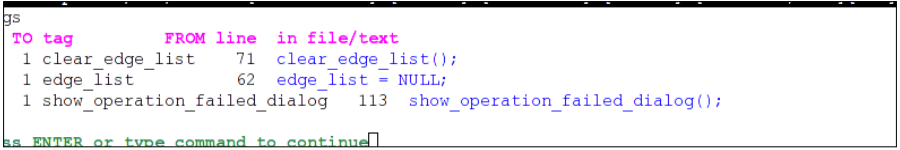
\includegraphics[scale=0.5]{./images/page82.png}
\end{center}
上图中以 \texttt{>} 开始的行是当前所在的 tag. 除了组合键 \key{Ctrl+]}
与 \key{Ctrl+t}, 还可以用下面这两个命令完成同样的功能:
\begin{itemize}
    \item \texttt{:tag}: 跳转到这个 tag
    \item \texttt{:pop}: 回到上一个 tag
\end{itemize}

如果匹配的 tag 比较多, 要是能把这些 tag 以列表的形式罗列出来可能会比较方便.
为了得到这个列表, 可以用下面两个命令中的任意一个:
\begin{itemize}
    \item \texttt{:tselect}
    \item \texttt{:ptselect}
\end{itemize}
第 1 个命令列出所有匹配的 tag, 为了选择其中一个, 需要输入 tag 所在行的行首的
数字.

第 2 个命令完成同样的工作, 但是它会在预览窗口中显示列表. 如果用户选错了 tag,
或者是想查看列表中的下一个 tag, 可以用下面的命令在 tag 间移动:
\begin{itemize}
    \item \texttt{:tnext}: 移动到列表中的下一个 tag
    \item \texttt{:tprev}: 移动到列表中的前一个 tag
\end{itemize}

用户可能还没有从前面的例子中体会到 tag list 的强大之外, 想像一下, 假设项目中的
文件不只 3 个, 而是散布在数百个目录中的上千个文件, 这时候, 用户肯定没办法记住
每个函数所在的位置, 这时候就非常需要一个强大的索引工具, 就像 tag list.
\marginpar{83}
\subsection{更便捷的 taglist 导航}
\label{subsec:easier_taglist_navigation}

在大多数的非英文键盘布局中, 按键 \texttt{]} 无法直接使用, 必须通过其他的组合
键 --- 比如 \key{Ctrl+Alt+G+r+9} --- 来完成 \key{Ctrl+]} 的功能. 在这种情况下,
把命令映射到直接可用的按键上会更方便一点, 对此, 笔者使用了下面的映射:
\begin{vimcode}
:nmap <buffer> <F7> <C-]>
:nmap <buffer> <C-F7> <C-T>
:nmap <buffer> <A-F7> :ptselect<cr>
:nmap <buffer> <F8> :tnext<cr>
:nmap <buffer> <C-F8> :tprev<cr>
\end{vimcode}
现在, 用户可以用 \key{F7} 与 \key{Ctrl+F7} 在 tag 间跳转, 用 \key{Alt+F7}
获取 tag 列表, 用 \key{F8} 与 \key{Ctrl+F8} 遍历 tag.

\subsection{taglist 的其他用法}
\label{subsec:other_usages_of_taglists}

Taglist 不仅可以用来查找函数与变量的定义, 还可以用来查找其他信息. 笔者在这里只
是简单地提一下 taglist 在 Vim 中的其他应用:
\begin{itemize}
    \item \texttt{lookupfile.vim}: 由 Hari Krishna Dara 开发, 该脚本使用 tag
        list 在一个预处理过的项目中查找指定的文件, 脚本的最新版见
        \url{http://www.vim.org/scripts/script.php?script_id=1581}.
    \item \texttt{taglist.vim}: 由 Yegappan Lakshmanan 开发的插件, 在程序员中
        非常流行. 它是一个完整的源代码浏览工具, 在一个分割的窗口中显示函数,
        关键词, 变量, 定义的概览. 插件的下载地址是
        \url{http://www.vim.org/scripts/script.php?script_id=273}.
    \item \texttt{ctags.vim}: 由 Gary Johnson 与 Alexey Marinichev 开发.
        脚本可以在状态条或窗口标题栏中显示光标所在位置的函数的名字. 脚本使用
        Exuberant Ctags 为当前打开的文件自动生成 tag 文件. 脚本的下载地址是
        \url{http://www.vim.org/scripts/script.php?script_id=610}.
    \item \texttt{autoproto.vim}: Jochen Baier 专门为 C 程序员开发的脚本. 当
        程序员输入函数名与第一个左括号后, 脚本在预览窗口中显示该函数的原型.
        脚本的下载地址是
        \url{http://www.vim.org/scripts/script.php?script_id=1553}.
\end{itemize}
\marginpar{84}
\begin{warning}
    关于 tag 的更多信息与使用方法, 可以查阅 Vim 的帮助系统 \texttt{:help tags}.
\end{warning}

\section{使用自动补全}
\label{sec:using_autocompletion}

作为一个遵循 Vim 哲学的用户, 总是希望用最少的击键来完成一件事, 因为额外的击键
意味着额外的时间.

所以说, 如果 Vim 可以猜出我们正想打的单词, 并且可以自动补全, 那我们又何必每次
都从头输到尾呢?

在 Vim 中有多种办法来自动补全单词, 其中一些只能补全用户曾经在某个打开的缓冲区
中输过的单词, 还有一些牵涉到了对当前正在使用的代码的分析 --- 不仅仅是当前打开
文件, 还包括整个源代码树.

在接下来的小节里, 我们将会讨论使用自动补全的三种方法:
\begin{itemize}
    \item 已知单词的自动补全
    \item 基于字典文件的补全
    \item 识别上下文的自动补全
\end{itemize}
除此之外, 我们还会介绍一些使用技巧, 通过按键绑定来更方便地使用自动补全.

\subsection{已知单词的自动补全}
\label{subsec:autocompletion_with_known_words}

在这一节, 我们将会看到自动补全的最简单的用法 --- 为已知单词进行补全.

无论用户在写什么内容, 都会出现输入重复单词的情况. 在 Vim 中, 用户可以在输入
完单词的头两个字母后, 按下组合键 \key{Ctrl+n}.
\marginpar{85}

示例:

假设用户想要在 Vim 中输入 ``I have beautiful flowers in my flower garden''.

在刚开始时, 文件中没有任何其他的内容, 因此用户不得不一个字母一个字母地写下
文本的开始部分, 直到 ``I have beautiful flowers in my f''.

用户接下来会输入单词 ``flower'', 但是, 由于我们在前面已经输入了 ``flowers'',
当输入 ``f'' 后, 按下 \key{Ctrl+n}, Vim 就会把 ``f'' 自动扩展为 ``flowers'',
我们只要把多余的 ``s'' 删掉即可. 和输入整个单词相比, 这要快很多.

随着文本的增多, 你会发现越来越多的单词可以自动补全.

组合键 \key{Ctrl+n} 所做的工作是向前搜索匹配的单词. 如果用户知道自己刚刚才输入
过同样的单词, 那么用 \key{Ctrl+p} 会更快一点, 因为这个组合键是向后搜索匹配.
一般来说, 除非文件非常大, 或者可能的匹配非常多, 否则 \key{Ctrl+n} 与
\key{Ctrl+p} 对用户来说并没有太大的区别.

\subsection{使用字典的自动补全}
\label{subsec:autocompletion_using_dictionary_lookup}

一个比较好的使用技巧是把用户所使用的语言的全部单词, 都搜集到一个巨大的字典
文件中, 然后再把这个文件作为字典加载到 Vim 中 (在因特网上很容易搜索到这种文件).
为了把文件作为字典载入到 Vim 中, 执行下面的命令:
\begin{vimcode}
:set dictionary+=/path/to/dictionary/file/with/words
\end{vimcode}
现在, Vim 已经事先知晓了大量的单词, 用户可以利用这些单词进行自动补全. 不过,
有一些地方会不一样. 因为补全时被搜索的单词并非在某个打开的缓冲区中, 而是 
在选项 \texttt{dictionary} 所配置的字典文件中, 所以需要用另一个快捷键:
\key{Ctrl+x+k}.
\marginpar{86}
按下 \key{Ctrl+x} 后, 会进入补全模式, 再接着按下 \key{Ctrl+k}, 就可以在字典中
查询关键词 (\key{k} 指是的是 keyword).
\begin{center}
    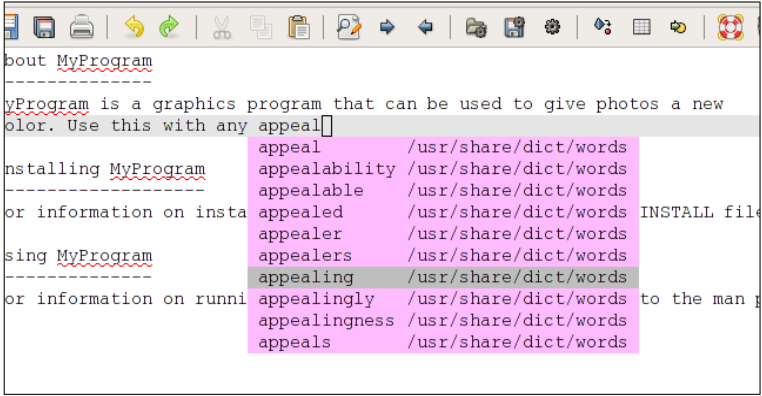
\includegraphics[scale=0.6]{./images/page86.png}
\end{center}

还有其他几种补全类型, 包括:

\key{Ctrl+x} 后跟:
\begin{itemize}
    \item \key{Ctrl+l}: 补全一整行文本
    \item \key{Ctrl+n}: 从当前缓冲区中补全单词
    \item \key{Ctrl+k}: 从字典中补全单词
    \item \key{Ctrl+t}: 从同义词典中补全单词 (见 \texttt{:help 'thesaurus'}
    \item \key{Ctrl+i}: 从当前文件与被包含的文件中补全单词
    \item \key{S}: 拼写建议 (仅 Vim 7.0 以上的版本支持)
\end{itemize}

其他的将会在下节介绍.

\subsection{omnicompletion}
\label{subsec:omnicompletion}

哪些内容应该自动补全, 哪些内容不应该自动补全 --- 对此我们都有完美的解决办法.
但是对于 Vim 来说, 在 7.0 版出现之前, 用户对补全并没有绝对的控制权.

Vim 7.0 引入了一种全新的补全技术 --- omnicompletion. 它使得用户可以精确地定义
补全功能应该如何工作. 实际上, 用户需要自己来编写补全函数 (除非已经有人把函数
写好了).
\marginpar{87}
和前一节介绍的一样, 激活补全的方法是先输入几个字母, 按下 \key{Ctrl+x} 进入到
补全模式, 再紧接着按下 \key{Ctrl+o} 使用 omnicompletion.

为了添加用户自定义的补全函数, 执行:
\begin{vimcode}
:set omnifunc=MyCompleteFunction
\end{vimcode}
现在, 你只需要定义函数 \texttt{MyCompleteFunction}, 这个函数用于完成补全操作.
上面的命令只在当前活动缓冲区内才有效, 如果希望每个缓冲区都可以使用该补全函数,
那么就要对每个缓冲区执行这个设置命令.
\begin{warning}
    \texttt{omnifunc} 的设置通常在文件类型插件内完成, 这样的话, 补全函数就可以绑
    定到特定的文件类型上.
\end{warning}

现在让我们来看一个补全函数的例子. 假设你有一个通讯录文件, 文件的内容是人名及其邮件
地址, 就像:
\begin{vimcode}
Kim Schulz|kim@schulz.dk
John Doe|john.doe@somedomain.com
Jane Dame|jd@somedomain2.com
Johannes Burg|jobu@somedomain3.net
Kimberly B. Schwartz|kbs@somedomain.com
\end{vimcode}

现在, 你想在写完一个人名后, 通过补全插入对应的邮件地址, 完成这个功能的函数是:
\begin{vimcode}
function! CompleteEmails(findstart, base)
	  if a:findstart
	    " locate the start of the word
	    let line = getline('.')
	    let start = col('.') - 1
	    while start > 0 && line[start - 1] =~ '\a'
	      let start -= 1
	    endwhile
	    return start
	  else
	    " find contact names matching with "a:base"
	    let res = []
		 " we read contactlist file and sort the result
	    for m in sort(readfile('/home/kim/.vim/contacts.txt'))
	      if m =~ '^' . a:base
				let contactinfo = split(m, '|')
\end{vimcode}
\marginpar{88}
\begin{vimcode}
		      " show names in list, but insert email address 
		      call add(res, {'word': contactinfo[1], 
                     \ 'abbr': contactinfo[0].' <'.contactinfo[1].'>',
                 \ 'icase': 1} )
	      endif
	    endfor
	    return res
	  endif
	endfunction
\end{vimcode}

函数接收两个参数 --- 所有的 omnicompletion 函数都是如此. Vim 第一次调用函数时,
把第 1 个参数 \texttt{findstart} 设置为 1 (\texttt{base} 为空). 这样的参数状态
表示这是第一次调用, 函数应该搜索用户当前所写的单词的开始.

然后, Vim 再次调用函数, 这次调用把 \texttt{findstart} 设置为 0, 把 \texttt{base}
设置成开始补全的单词. 这一次, 函数会打开通讯录文件, 以行为单位, 把文件读到
一个列表中, 对列表排序, 然后遍历列表.

每一行的内容按照 \texttt{|} 分割, 如果某个单词, 是以用于补全的单词的字母作为开
始, 那就把这个单词添加到结果列表中, 这个结果列表最后会作为函数的返回值返回.
函数可以修改弹出内容的外观, 和它所匹配的内容, 这两个功能无法通过添加电子邮件
地址来完成, 而是要通过构建一个字典 (见 \texttt{:help Dictionary}), 在构建字典
时会接触到一些特定的关键词. 在这个案例中, 我们使用下列三个关键词:
\begin{itemize}
    \item Word: 应该插入的真正的单词
    \item Abbr: 在弹出列表中使用的单词, 而非直接使用 word
    \item Icase: 如果其值非零, 则匹配是区分大小写的
\end{itemize}

其他的关键词及其意义可以在 Vim 的帮助系统中找到:
\begin{vimcode}
:help 'omnifunc'
\end{vimcode}

现在 Vim 已经有了一个单词列表用于补全, 在这个案例中则是一些像下面这样的行:
\begin{vimcode}
"Kim Schulz <kim@schulz.dk>"
\end{vimcode}
无论何时写下一些字母,比如 \texttt{ki}, 然后按下 \key{Ctrl+x Ctrl+o}, Vim 就会 
以列表的形式, 弹出所有的, 以 \texttt{ki} 开始的名字.
\marginpar{89}
\begin{center}
    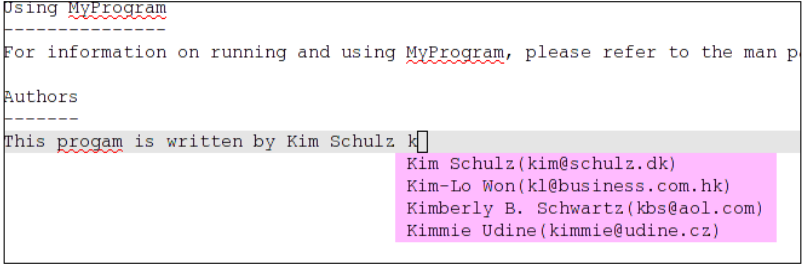
\includegraphics[scale=0.55]{./images/page89.png}
\end{center}
按 \key{Ctrl+o} 可以循环遍历列表中的条目. 另外, 还可以用 \key{Ctrl+n} 向前遍历,
用 \key{Ctrl+p} 向后遍历.

\subsection{多合一补全}
\label{subsec:all_in_one_completion}

用户可能不想记住这么多的补全快捷键, 为什么就不能为所有的补全类型只使用一个快捷
键呢? Vim 可以帮助你实现这个愿望, 让我们来看一下具体要怎么做.

大部分支持补全的编辑器通常把这个功能映射到 \key{Tab} 键.

通过下面这个命令, 用户可以在 Vim 的帮助系统中找到一个叫作
\texttt{CleverTab()} 的函数:
\begin{vimcode}
:help ins-completion
\end{vimcode}
这个函数可以让用户使用 \key{Tab} 键来补全单词, 而非 \key{Ctrl+n}. 函数可以自动
区分是应该插入一个制表符, 还是应该做补全操作. 如果用户是在一行的开始, 或者是 
某个空白符的后面按下 \key{Tab} 键, 那就是插入一个制表符. 在其他的情况下, 函数 
会试图完成已知单词的补全.

我们借用帮助系统中的 \texttt{CleverTab} 函数, 并对它加以扩展, 使得它可以从下
面的, 带有优先级的列表中选择补全方法:
\begin{itemize}
    \item omnicompletion
    \item 字典补全
    \item 已知单词的补全
\end{itemize}
\marginpar{90}
下面是实现该函数的一个例子:
\begin{vimcode}
function! SuperCleverTab()
	'check if at beginning of line or after a space
    if strpart( getline('.'), 0, col('.')-1 ) =~ '^\s*$'
      return "\<Tab>"
    else
		" do we have omni completion available
       if &omnifunc != ''
		" use omni-completion 1. priority
          return "\<C-X>\<C-O>"
       elseif &dictionary != ''
			" no omni completion, try dictionary completio
			return "\<C-K>"
		else
			"use omni completion or dictionary completion
			"use known-word completion
          return "\<C-N>"
      endif
    endif
endfunction

" bind function to the tab key
inoremap <Tab> <C-R>=SuperCleverTab()<cr>
\end{vimcode}

把函数的代码与按键绑定添加到 \texttt{vimrc} 中, 然后你就可以用 \key{Tab} 键来 
完成各种类型的补全.

按下 \key{Tab} 键进行补全时, 函数检查此时是否是要插入一个制表符. 如果不是, 那
就检查 omnicompletion 函数 (通过 \texttt{omnifunc} 设置) 是否可用. 如果函数不
可用, 那就检查字典是否可用. 如果字典还是不可用, 那就使用最简单的已知单词补全.

\section{宏录制}
\label{sec:using_macro_recording}

编辑具有单一结构的文本时, 或许最好的功能就是录制一段输入宏, 然后再重复执行宏.

完成这个工作的接口非常简单, 更强大的是, 几乎任何东西都可以录制, 接下来我们就
来介绍这个强有力的工具.
\marginpar{91}

让我们先来看一下将会用到的命令:
\begin{itemize}
    \item \texttt{qa}: 从现在开始录制, 并记录到寄存器 \texttt{a}. 可以使用任意
        的寄存器, 用寄存器 \texttt{a} 只是为方便起见.
    \item \texttt{q}: 如果是在正在录制时按下, 则停止录制
    \item \texttt{@a}: 执行记录在寄存器 \texttt{a} 中的宏 (可以把 \texttt{a}
        替换成其他的寄存器)
    \item \texttt{@@}: 执行上一次所执行的宏命令
\end{itemize}
可以在 \texttt{@} 前加上任意的数字, 表示重复执行该命令多少次. 例如,
\texttt{15@a} 表示把寄存器 \texttt{a} 中所记录的命令重复执行 15 遍.

现在让我们看一下一次普通的录制会话:
\begin{vimcode}
qq
command1
command2
....
commandN
q
10@q
\end{vimcode}
读者可能会好奇这有什么用, 因为这只是在重复执行一串命令罢了. 这种问题最好通过
例子来说明.

想像一下你有一大串的信息需要处理, Unix 系统的日志文件就属于这种类型. 日志文件
的内容类似于:
\begin{vimcode}
Mar 20 17:23:54 Inspiron kernel: [33604.866998] ath9k 0000:09:00.0: no hotplug settings from platform
Mar 20 17:23:54 Inspiron kernel: [33604.867007] pcieport 0000:00:1c.7: no hotplug settings from platform
Mar 20 17:23:54 Inspiron kernel: [33604.867015] ehci-pci 0000:00:1d.0: no hotplug settings from platform
Mar 20 17:23:54 Inspiron kernel: [33604.867020] ehci-pci 0000:00:1d.0: using default PCI settings
Mar 20 17:23:54 Inspiron kernel: [33604.867039] lpc_ich 0000:00:1f.0: no hotplug settings from platform
Mar 20 17:23:54 Inspiron kernel: [33604.867043] lpc_ich 0000:00:1f.0: using default PCI settings
Mar 20 17:23:54 Inspiron kernel: [33604.867063] ahci 0000:00:1f.2: no hotplug settings from platform
Mar 20 17:23:54 Inspiron kernel: [33604.867067] ahci 0000:00:1f.2: using default PCI settings
Mar 20 17:23:54 Inspiron kernel: [33604.867084] pci 0000:00:1f.3: no hotplug settings from platform
Mar 20 17:23:54 Inspiron kernel: [33604.867089] pci 0000:00:1f.3: using default PCI settings
...
\end{vimcode}
\marginpar{92}

现在, 用户想要把这个日志文件转换成 HTML, 并以表格的形式呈现数据, 看起来就像:
\begin{vimcode}
<tr><td>Oct 8 21:23:34</td><td>laptopia</td><td>kernel:</td><td>ACPI...</td><tr>
\end{vimcode}

用户可以选择一行一行地编辑文件, 直到最后一行. 但也可以这样做, 先编辑一行, 并把 
编辑命令录制下来, 然后再把录制下来的命令应用到剩下的每一行. 最开始的编辑命令可
以是下面这些 (假设光标原来是在第一行的开始):
\begin{center}
    \begin{tabular}{ll}
    \hline
    \texttt{qa}             & 开始录制, 并把内容记录到寄存器 \texttt{a} 中 \\
    \texttt{i<tr><td>[ESC]} & 切换到插入模式, 插入 HTML 标记, 再回到普通模式 \\
    \texttt{/ [CR]}         & 向前搜索空格 \\
    \texttt{3n}             & 向前搜索到第 3 个空格 \\
    \texttt{xi</td><td>[ESC]}& 删除空格, 切换到插入模式, 添加 HTML 标记, 再切换
        到普通模式 \\
    \texttt{n}              & 前进到下一个空格 \\
    \texttt{xi</td><td>[ESC]}& 删除空格, 切换到插入模式, 添加 HTML 标记, 再切换
        到普通模式 \\
    \texttt{n}              & 前进到下一个空格 \\
    \texttt{xi</td><td>[ESC]}& 删除空格, 切换到插入模式, 添加 HTML 标记, 再切换
        到普通模式 \\
    \texttt{A</td></tr>[ESC]}&在行的末尾添加 HTML 标记, 再切换到普通模式 \\
    \texttt{j\^}            & 前进到下一行的开始 \\
    \texttt{q}              & 宏录制结束 \\
    \hline
\end{tabular}
\end{center}

\begin{warning}
    \texttt{[ESC]} 指的是按下转码键: \key{Esc}, \texttt{[CR]} 指的是按下回车键:
    \key{Enter}.
\end{warning}

现在我们已经准备好了完整的宏, 光标的位置也已就位, 这意味着我们现在可以重复地
执行宏, 并且在每次执行完宏后, 光标都会处在就绪的位置下.

用户可以用 \texttt{@a} 来回放存放在寄存器 \texttt{a} 中的宏, 除此之外, 用户还 
需要做的就是添加 HTML 的头部与尾部信息, 这很简单.
\marginpar{93}
这只是宏应用的一个简单示例, 如果读者认真回忆一下, 可能会想到更多的, 可以用宏
来优化的工作.

\section{使用会话}
\label{sec:using_sessions}

不知读者有没有想过, Vim 会为你保存多少信息. Vim 保存的信息涵盖了大量的内容, 其
中包括:
\begin{itemize}
    \item 打开的文件, 缓冲区, 窗口, 和标签页
    \item 历史命令
    \item 文本的变化点
    \item 选择与撤消分支
    \item 窗口, 分割 与 GUI 窗口的大小
    \item 光标的位置
\end{itemize}

保存的信息可以分为三类:
\begin{itemize}
    \item 第一类设置信息称为视图 (view), 该类信息应用到一个单独的窗口上. 一个视
        图可以被存储和还原, 因此每当用户使用视图时, 窗口都会呈现出相同的外观.
    \item 第二类设置信息称为会话 (session). 它是一系列视图的集合, 再加上视图
        之间如何配合的信息. 和视图一样, 会话也可以保存下来, 以便于稍后检索.
    \item 剩下的其他信息都归为第三类, 也就是所有的, 不能直接应用到任意一个窗口
        的全局设置. 这些设置可以用会话保存下来, 因此它们也可以保存/还原.
\end{itemize}

在接下来的小节里, 我们将会介绍如何在日常的工作中运用会话.

\subsection{简单的会话使用}
\label{subsec:simple_session_usage}

在使用会话的过程中, 最经常做的事就是把当前正在运行的会话 (如果没有经过特别的设
置, 则是默认会话) 保存到会话文件中, 这样就可以在需要时重新加载会话. 保存会话
的命令是:
\begin{vimcmdform}
\texttt{:mksession}\ \textit{file}
\end{vimcmdform}
保存当前视图的命令是:
\begin{vimcmdform}
\texttt{:mkview}\ \textit{file}
\end{vimcmdform}
\marginpar{94}
命令中的 \textit{file} 是用户指定的, 用于保存会话或视图的文件名. 如果没有指定该
参数, 则默认保存到当前工作目录的 \texttt{Session.vim} 文件中.

\begin{warning}
    如果文件事先存在, 为了覆盖掉文件原来的内容, 需要在 \texttt{mksession} 的末
    尾紧跟上一个感叹号 \texttt{!}.
\end{warning}

使用视图时, 你可以同时拥有多个不同的视图. 如果每个视图都保存到当前工作目录下, 那
么不用多长时间, 工作目录就会被视图文件填满. 为了避免这个问题, 可以用下面的命令 
告诉 Vim, 应该把视图文件放到哪个目录下:
\begin{vimcode}
:set viewdir=$HOME/.vim/views
\end{vimcode}
上面的命令会把所有的视图文件保存到目录 \texttt{\$HOME/.vim/views}.

假设用户当前打开了三个窗口, 在退出 Vim 之前, 用户执行了:
\begin{vimcode}
:mksession
\end{vimcode}
在下一次准备打开文件时, 用户希望用相同的会话来启动 Vim, 此时可以用命令行选项
\texttt{-S}:
\begin{vimcode}
vim -S Session.vim
\end{vimcode}

除此之外, 用户也可以选择在启动 Vim 后, 用下面的命令来加载会话文件:
\begin{vimcode}
:source Session.vim
\end{vimcode}

对于视图, 加载方式是:
\begin{vimcode}
:loadview View.vim
\end{vimcode}

加载一个会话会改变编辑器的整体布局, 而加载一个视图则只会改变当前活动窗口的布局.
\marginpar{95}
\begin{warning}
    用户如果希望 Vim 记住所有的设置信息, 比如光标的位置与折叠信息, 那么就需要在
    \texttt{vimrc} 中添加如下内容:
    \begin{vimcode}
    set viewdir=$VIMHOME/views/
    autocmd BufWinLeave * mkview
    autocmd BufWinEnter * silent loadview
    \end{vimcode}
    无论何时在同一个窗口中打开另一个缓冲区, 之前的缓冲区的视图都会被自动保存下来,
    并且当再次打开之前的缓冲区时, 会自动还原保存的视图.
\end{warning}

会话的一个常用技巧是定义一个命令, 命令的功能是在退出 Vim 时自动保存会话, 而在打开 Vim
时自动还原保存的会话. 使用这个方法就可以让用户在不丢失设置, 已打开文件列表等
信息的前提下, 自由地启动与退出 Vim. 为了完成这个功能, 可以在 \texttt{vimrc} 中
添加如下命令:
\begin{vimcode}
autocmd VimEnter * call LoadSession()
autocmd VimLeave * call SaveSession()
function! SaveSession()
   execute 'mksession! $HOME/.vim/sessions/session.vim'
endfunction

function! LoadSession()
   if argc() == 0
      execute 'source $HOME/.vim/sessions/session.vim'
   endif
endfunction
\end{vimcode}
关闭 Vim 后, 会话保存到 \texttt{\$HOME/.vim/sessions/session.vim}.

根据打开 Vim 方式的不同, 或者是打开由命令行参数指定的文件, 或者是打开最后一次
会话. 比如说:
\begin{itemize}
    \item \texttt{vim file.txt}: 这种打开方式不会加载最后一次会话.
    \item \texttt{vim}: 这种打开方式会加载最后一次会话, 之前打开的文件会再次
        被打开.
\end{itemize}

如果你希望在会话文件中存放更多的信息, 可以把额外的信息存放到额外的会话文件中.
方法是创建一个其名字类似于会话文件的文件, 不过要把扩展名 \texttt{.vim} 改成
\texttt{x.vim}. 例如, \texttt{Session.vim} 的额外会话文件是
\texttt{Sessionx.vim}. 额外的会话文件应该和其所属的会话文件放在同一目录下. 你
可以把你想要添加的命令全写到这个文件中, 当 Vim 加载会话文件时, 会把额外的会话
文件中的命令执行一遍.
\marginpar{96}

\subsection{满足个人的会话需求}
\label{subsec:satify_you_own_session_needs}

用户可能并不需要会话文件中存放的所有信息, 有时, 用户可能仅仅是想要保存打开过
的文件的信息, 而在其他时候, 可能是所有的会话信息. 幸运的是, Vim 提供了设置
保存会话信息的方法.

所使用的设置命令是 \texttt{sessionoptions}, 使用方法是:
\begin{vimcmdform}
\texttt{:set sessionoptions=}\textit{options}
\end{vimcmdform}
\textit{options} 是一个由逗号分隔的列表, 列表中可以出现下列选项:
\begin{center}
    \begin{tabular}{lp{35em}}
        \hline
        \textbf{\texttt{blank}}  & 保存空白窗口 \\
        \textbf{\texttt{buffers}} & 保存所有缓冲区的信息, 包括隐藏的与未加载的缓冲区 \\
        \textbf{\texttt{curdir}} & 保存当前工作目录的相关信息 \\
        \textbf{\texttt{folds}} & 保存缓冲区内容中的折叠信息 \\
        \texttt{globals} & 保存全局变量的相关信息, 这里的全局变量指的是以大写
        字母开始, 且类型为字符串或数值的变量 \\
        \textbf{\texttt{help}} & 保存帮助窗口 \\
        \texttt{localoptions} & 保存用户在单个窗口中创建的局部变量与局部映射的
        相关信息 \\
        \textbf{\texttt{options}} & 保存所有的选项信息, 包含全局的与局部的 \\
        \texttt{resize} & 保存 UI 窗口的尺寸信息 (行数与列数) \\
        \texttt{sesdir} & 如果设置了该选项, 当前目录就会是会话文件的存放目录
        (如果同时设置了 \texttt{curdir}, 则该选项不可用) \\
        \texttt{slash} & 把所有文件路径中的反斜杆换成斜杆 (这样做就可以让 Unix
        兼容 Windows 的文件路径) \\
        \textbf{\texttt{tabpages}} & 保存所有的标签页信息, 如果没有设置该选项, 则只会保
        存当前处于活跃状态的标签页 \\
        \texttt{unix} & 使用 Unix 格式的行结束符, 而非 Windows 格式 \\
        \texttt{winpos} & 保存 UI 窗口的屏幕位置信息 \\
        \textbf{\texttt{winsize}} & 保存所有打开窗口的尺寸 \\
        \hline
    \end{tabular}
\end{center}
\marginpar{97}
